\textbf{COLUNI 2026 -- Questão 05}\par\medskip \textbf{Leia os textos III e IV para responder às questões 5, 6 e 7:}

\textbf{Texto III}

Foi uma moça lavar suas anáguas no rio. Espuma de rendas, espuma de águas. Depois deitou-as sobre a grama para secar. E da grama uma salamandra levantou a cabeça e perguntou:

- Que rendas são essas que você lava com tanto capricho?

- São as rendas que farfalham nos meus tornozelos - respondeu a moça.

- Eu também quero ouvir esse farfalhar - disse a salamandra. E antes mesmo que a moça vestisse a primeira anágua, enroscou-se no seu tornozelo.

Era fria como o vidro e brilhante como a prata. Mas, com medo de ser mordida, a moça deixou-a estar e voltou para a aldeia. No caminho encontrou as outras moças da sua rua, que iam juntas. - Que joia tão diferente! - exclamaram, flagrando nos passos dela o luzir da salamandra. - Onde foi que você achou?

A moça riu sem responder, entrou em casa e fechou a porta atrás de si.

\begin{flushright}(COLASSANTI, Marina. \textbf{Com certeza tenho amor}. São Paulo: Global, 2009. p. 61.)\end{flushright}

\textbf{Texto IV}

% COLUNI-AUTO-FIGURES-BEGIN
\begin{figure}[htbp]
\centering
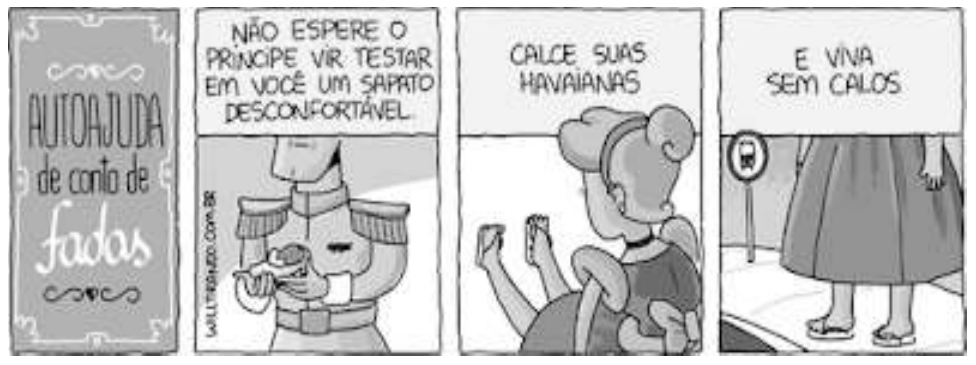
\includegraphics[width=0.75\linewidth]{static/simulados/coluni/figuras/2026/questao-05/figura-1.png}
\end{figure}
% COLUNI-AUTO-FIGURES-END
\begin{center}(Disponível em: https://volk-lore.blogspot.com/2019/01/autoajuda-de-conto-de-fadas_30.html. Acesso em: 15 ago. 2025)\end{center}

De acordo com a análise dos textos III e IV, é INCORRETO afirmar que:
\begin{enumerate}
\item São constituídos em uma esfera de encantamento, através de uma linguagem denotativa.
\item Fazem parte do mundo “fantástico”, oscilando entre real e imaginário, mistura de insólito e de cotidiano.
\item Recuperam o cenário dos contos de fadas, mas conferem-lhe um novo estilo linguístico e ficcional.
\item Instauram uma reflexão que articula conflitos cotidianos e o extraordinário da realidade.
\end{enumerate}
